\section{Auswertung}
\label{sec:Auswertung}
\subsection{Bestimmung der Kraftflussdichte}
Die mit der Hallsonde aufgenommenen Messwerte für die Ortsabhängigkeit der magnetischen Flussdichte $B(z)$ sind in Tabelle \ref{tab:messwerte} aufgelistet sowie in Abb.\ref{fig:b-feld} graphisch dargestellt. Es ist zu erkennen, dass die Flussdichte ihr Maximum bei $z = \SI{0}{\milli\meter}$ hat und ihr Wert beträgt hier $\SI{467}{\milli\tesla}$. Dabei ist der Ort der maximalen Kraftflussdichte $B(z)$ die Position der Probe. Dabei ist $z= \SI{0}{\milli\meter}$ keine ausgezeichnete Position der Hallsonde, sondern eine willkürliche ausgewähle Position in Probennähe.

\begin{table}[htpb]
	\centering
	\caption{Die Messwerte für die Kraftflussdichte $B(z)$ in Abstand $z$ bzw. in der Nähe der Probenposition.}
	\label{tab:messwerte}
	\begin{tabular}{r|r|r|r}
		\toprule
		$z/\si{\milli\meter}$	&	$B(z) / \si{\milli\tesla}$ &	$z/\si{\milli\meter}$ &  $B(z) / \si{\milli\tesla}$\\
		\hline
		-29	&	1 &2&460\\
		-24	&	4 &4&444\\
		-22	&	8 &6&412\\
		-20	&	14&8&345\\
		-18	&	28&10&237\\
		-16	&	52&12&123\\
		-14	&	115&14&63\\
		-12	&	217&16&33\\
		-10	&	355&18&18\\
		-8	&	415&20&9\\
		-6	&	446&22&5\\
		-4	&	461&24&3\\
		-2	&	466&26&1 \\
		0   &   467&&\\
		\bottomrule
	\end{tabular}
\end{table}

\begin{figure}[h!]
	\centering
	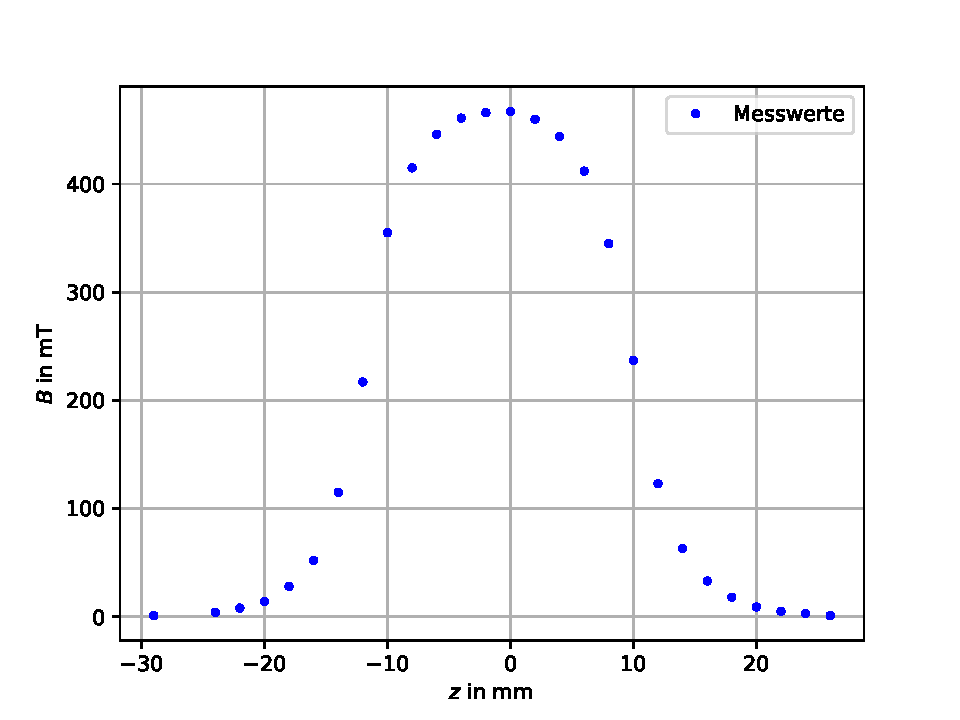
\includegraphics[width=0.7\linewidth]{../../B-Feld}
	\caption{Ortsabhängigkeit der magnetischen Flussdichte $B(z)$.}
	\label{fig:b-feld}
\end{figure}

\subsection{Die Faraday Rotation}
Im nächsten Versuchsteil wird die Faraday-Rotation für zwei unterschiedliche Galliumarsenid-Proben untersucht. Die Eigenschaften der Proben sind in der Tabelle \ref{tab:messwerte1} zu finden. Es werden jeweils für die Berechnung der Drehwinkel, zwei Winkel für verschiedene Wellenlängen im nahen Infrarotbereich ($\SI{1,06}{\micro\meter}$ - $\SI{2,65}{\micro\meter}$) aufgenommen. Der Winkel $\theta_{1}$ ist der Winkel, der vor der Umpolung aufgenommen wird und der Winkel $\theta_{2}$ wird nach der Umpolung aufgeschrieben. Die jeweiligen Messwerte für $\theta_{1}$ und $\theta_{2}$ sind in Tabelle \ref{tab:messwerte2} enthalten. 

\begin{table}[htpb]
	\centering
	\caption{Dotierung $N$ und die Probendicke $L$ der untersuchten GaAs-Proben.}
	\label{tab:messwerte1}
	\begin{tabular}{r|r|r}
		\toprule
		Bezeichung GaAs-Proben & $N / \frac{1}{\si{\cubic\centi\meter}}$	&	$L / \si{\milli\meter}$ \\
		\midrule
		hochrein & - & 5,11 \\
		schwach dotiert & 1,28 $\cdot 10^{18}$ & 1,36 \\
		\bottomrule
	\end{tabular}
\end{table}

Der gesamte Drehwinkel der Faraday-Rotation wird dann mittels Gleichung \ref{eq:drehwinkeldifferenz} berechnet, da die Proben verschiedene Dicken aufweisen (s.Tabelle \ref{tab:messwerte1}) und um die verschiedenen Proben vergleichen zu können, müssen die Winkel auf die entsprechenden Probenlängen normiert werden. Die Ergebnisse der Messung sind in der Tabellen \ref{tab:messwerte2} und \ref{tab:messwerte4} zu finden und die Werte für den Drehwinkel pro Rad werden in der Abbildung \ref{fig:messdaten} aufgetragen.

\begin{equation}
\label{eq:drehwinkeldifferenz}
\theta_\text{n} = \frac{\theta_{1}-\theta_{2}}{2L}
\end{equation}

\begin{table}[htpb]
	\centering
	\caption{Die aufgenommenen Winkel in Abhängigkeit der Wellenlängen für die GaAs-Proben.}
	\label{tab:messwerte2}
	\begin{tabular}{r|rr|rr}
		\hline\hline
		&	\multicolumn{2}{c|}{GaAs$_\text{hr}$}&	\multicolumn{2}{c|}{GaAs$_\text{sw}$} \\ 
		$\lambda / \si{\micro\meter}$ & $\theta_{1} / ^\circ$  & $\theta_{2} / ^\circ$ & $\theta_{1} / ^\circ$ & $\theta_{2} / ^\circ$ \\
		\hline\hline
		1,06	&	288,20	&	313,00	&	294,67	&	297,22	\\
		1,29	&   304,52	&	286,52	&	300,00	&	293,00  \\
		1,45	&	302,58  &	288,00	&	304,33	&	288,16	\\
		1,72	&   301,65	&	290,00	&	294,00	&	298,33	\\
		1,96	&	299,58	&	291,25	&	295,08	&	297,22	\\
		2,34	&	306,50	&	303,42	&	312,83	&	309,00	\\
		2,65	&	309,00  &	298,50	&	321,33	&	311,50	\\
		\hline\hline
		&	\multicolumn{2}{c|}{GaAs$_\text{hr}$}&	\multicolumn{2}{c|}{GaAs$_\text{sw}$} \\ 
		$\lambda / \si{\micro\meter}$ & $\theta_{1} /$ rad  & $\theta_{2} /$ rad & $\theta_{1} /$ rad & $\theta_{2} /$ rad \\
		1,06	&	5,03	&	5,46	&	5,14	&	5,18	\\
		1,29	&   5,31	&	5,00	&	5,23 	& 	5,11	\\
		1,45	&	5,28  	&	5,02	&	5,31	 &	5,03	\\
		1,72	&   5,26	&	5,06	&	5,13	 &	5,20	\\
		1,96	&	5,22	&	5,08	&	5,15	 &	5,18	\\
		2,34	&	5,34	&	5,29	&	5,45	 &	5,39	\\
		2,65	&	5,39    &	5,20	&	5,60	 &	5,43	\\
		\bottomrule
	\end{tabular}
\end{table}

%\begin{table}[htpb]
%	\centering
%	\caption{Normierter Drehwinkel $\theta_n$ in Abhängigkeit der Wellenlänge $\lambda$ und der Länge $L$ - zuerst in Grad ausgerechnet.}
%	\label{tab:messwerte3}
%	\begin{tabular}{ccc}
%		\toprule
%		& GaAs$_\text{hr}$ & GaAs$_\text{sw}$ \\
%		\midrule
%		$\lambda / \si{\micro\meter}$ & $\frac{\theta_n}{L}$ in $^{\circ}/\si{\milli\meter}$ & $\frac{\theta_n}{L}$ in $^{\circ}/\si{\milli\meter}$ \\
%		\midrule
%		1,06	& 2,42	& 0,93	\\
%		1,29	& 1,76	& 2,57	\\
%		1,45	& 1,42	& 5,94	\\
%		1,72	& 1,13	& 1,59	 \\
%		1,96	& 0,81	& 0,78	\\
%		2,34	& 0,30	& 1,40	 \\
%		2,65	& 1,02	& 3,61	\\
%	\bottomrule
%	\end{tabular}
%\end{table}

\begin{table}[htpb]
	\centering
	\caption{Normierter Drehwinkel $\theta_n$ in Abhängigkeit der Wellenlänge $\lambda$ und der Länge $L$ - in Rad ausgerechnet.}
	\label{tab:messwerte4}
	\begin{tabular}{ccc}
		\toprule
		& GaAs$_\text{hr}$ & GaAs$_\text{sw}$ \\
		\midrule
		$\lambda / \si{\micro\meter}$ & $\frac{\theta_n}{L}$ in $\frac{1}{\si{\milli\meter}}$ & $\frac{\theta_n}{L}$ in $\frac{1}{\si{\milli\meter}}$ \\
		\midrule
		1,06 	& 0,042	& 0,016 \\
		1,29	& 0,031	& 0,044 \\
		1,45	& 0,024	& 0,103 \\
		1,72	& 0,019	& 0,027 \\
		1,96	& 0,014	& 0,013 \\
		2,34	& 0,005	& 0,024 \\
		2,65	& 0,017 & 0,063	\\
		\bottomrule
	\end{tabular}
\end{table}

\begin{figure}[h!]
	\centering
	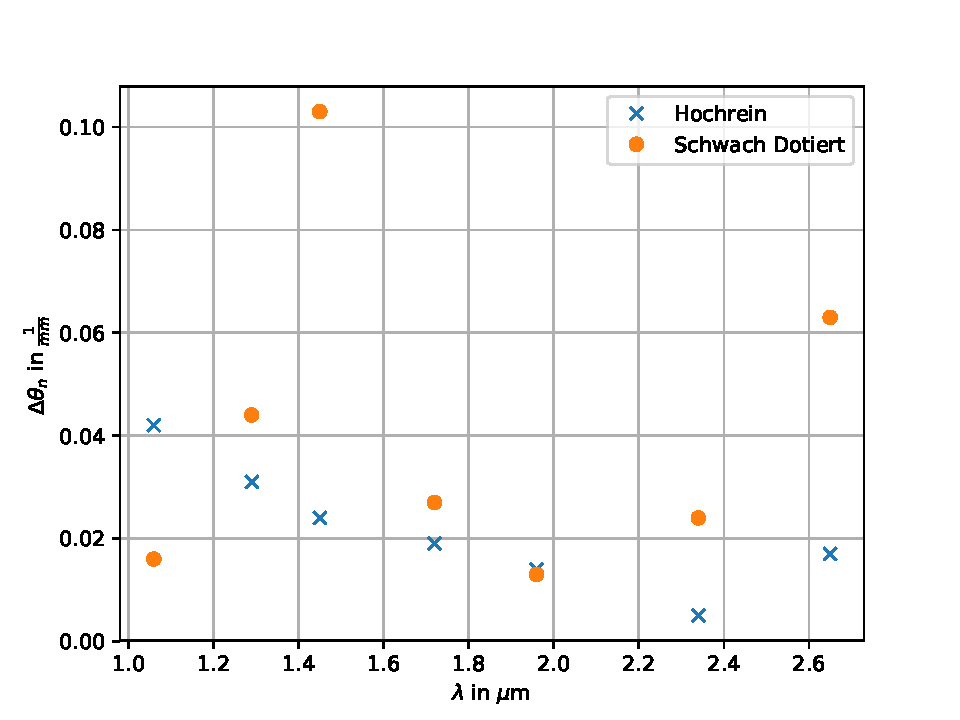
\includegraphics[width=0.7\linewidth]{../../Messdaten}
	\caption{Normierter Drehwinkel $\Delta\theta_\text{n}$ aufgetragen für alle untersuchten Proben in Abhängigkeit der Wellenlänge $\lambda$. Zu sehen ist, dass es sich bei der schwachen Dotierung kein linearer Zusammenhang ergeben hat und somit kein Verlauf existiert.}
	\label{fig:messdaten}
\end{figure}

\subsection{Bestimmung der effektiven Masse}
Für die Bestimmung der effektiven Masse der Elektronen im dotierten GaAs wird zuerst die Differenz der normierten Drehwinkel $\Delta\theta_\text{norm}$ zwischen der dotierten und hochreinen Probe wie folgt berechnet:
\begin{equation} 
\label{eq:differenznr}
\Delta\theta_\text{norm} = \theta_\text{n,dot} - \theta_\text{n,rein}
\end{equation}
In der Tabelle \ref{tab:messwerte5} ist die errechnete Differenz $\Delta\theta_\text{norm}$ für die schwache dotierte Probe aufgetragen. Mit Hilfe der folgenden Gleichung:
\begin{equation}
\label{eq:effektiveMasse}
\frac{\theta}{L} = \frac{e^3}{8\pi^2c^3\epsilon_0}\frac{1}{m^{*2}}\lambda^2\frac{NB}{bn} = a \cdot \lambda^2
\end{equation}
lässt sich die effektive Masse $m^*$ aus einer linearen Ausgleichsrechnung der Form:
\begin{equation}
\label{eq:ausgleichsgerade}
y = ax + b
\end{equation}
wobei $a$ die Steigung und $b$ der y-Achsenabschnitt sind, bestimmen, wenn $\frac{\Delta\theta_\text{norm}}{L}$ gegen $\lambda^2$ aufgetragen wird. Der y-Achsenabschnitt $b$ beträgt in diesem Fall den Wert $0$ und wird im weiteren Verlauf für die Berechnung der effektiven Masse vernachlässigt. Der Wert mit einem * aus der Tabelle \ref{tab:messwerte5} wird in der folgenden Ausgleichsrechnung nicht beachtet, da dieser stark von den sonstigen Messwerten abweicht. Mit der jeweiligen Steigung $a$ der Ausgleichsgeraden ergibt sich durch Vergleich mit der Gleichung \ref{eq:effektiveMasse} für die effektive Elektronenmasse:
\begin{equation}
\label{eq:eff2}
m^* = \sqrt{\frac{e^3NB}{8\pi^2\epsilon_0c^3na}}
\end{equation}
Über Formel \ref{eq:ausgleichsgerade} wird die Steigung und der Fehler der Ausgleichsgerade vom Python-Modul Scipy curve\_fit berechnet. 
Es wird $\frac{\Delta\theta_\text{norm}}{L}$ gegen $\lambda^2$ in die Abbildung \ref{fig:effektivemass1} aufgetragen und es ergibt sich für die Steigung $a$ der folgende Wert:
\begin{equation*}
a = \SI{0,003503 \pm 0,003041}{\radian\per\um\squared\per\mm} = \SI{3,503 \pm 3,041 E12}{\radian\cubic\per\m}
\end{equation*}
Der Fehler der effektiven Masse $\Delta m^*$ ergibt sich über die Gaußsche Fehlerfortpflanzung zu:
\begin{equation}
\label{eq:gaußfehler}
\Delta m^* = \frac{1}{2}\sqrt{\frac{e^3NB}{8\pi^2\epsilon_0c^3na^3}} \cdot \Delta a
\end{equation}
wobei $\Delta a$ der Fehler der Steigung $a$ aus der Ausgleichsrechnung ist. Es ergibt sich die hieraus nach Gleichung \ref{eq:eff2} berechnete effektive Masse (Fehler nach Gleichung \ref{eq:gaußfehler}) und das Verhältnis $\frac{m^*}{m_e}$ der berechnete effektive Masse zur Elektronenmasse\cite{Elektronenmasse} wie folgt:
\begin{align*}
m^* &= \SI{1,055 \pm 0,045 E-31}{\kilogram}\\ 
\frac{m^*}{m_e} &= 0,115 \pm 0,0049
\end{align*}
Für den wellenlängenabhängigen Brechungsindex $n$ von GaAs wird auf Grund der hohen Konstanz im Infraroten Bereich der Wert $n = 3,35$ für die weitere Berechnung festgelegt. Dieser ergibt sich aus den Daten\cite{GalliumArsenide} für eine Wellenlänge von $\lambda = \SI{1771,4}{\nano\meter}$, was in etwa der mittleren Wellenlänge während der Versuchsdurchführung entspricht.

\begin{table}[htpb]
	\centering
	\caption{Die Differenz der normierten Drehwinkel $\theta_n$ in Abhängigkeit der Wellenlänge $\lambda$ und der Länge $L$. Der Wert bei einer Wellenlänge von $\SI{1,45}{\micro\meter}$ mit * wird nicht bei der Ausgleichsrechnung beachtet.}
	\label{tab:messwerte5}
	\begin{tabular}{cc}
		\toprule
		& GaAs$_\text{sw}$ \\
		\midrule
		$\lambda / \si{\micro\meter}$ &  $\frac{\Delta\theta_\text{norm}}{L}$ in $\frac{1}{\si{\milli\meter}}$ \\
		\midrule
		1,06 	&  0,026 \\
		1,29	&  0,013 \\
		1,45	&  0,079* \\
		1,72	&  0,008 \\
		1,96	&  0,001 \\
		2,34	&  0,019 \\
		2,65	&  0,046 \\
		\bottomrule
	\end{tabular}
\end{table}

\begin{figure}[h!]
	\centering
	\includegraphics[width=0.7\linewidth]{../../EffektiveMass1}
	\caption{Lineare Ausgleichsrechnung für die Bestimmung der effektiven Elektronenmasse für die schwach dotierte Probe.}
	\label{fig:effektivemass1}
\end{figure}


